\documentclass[10pt,conference,a4paper]{IEEEtran}
\usepackage[utf8]{inputenc}
\usepackage{amsmath,amssymb}
\usepackage{graphicx}
\usepackage{booktabs}
\usepackage{microtype}
\usepackage{cite}
\usepackage{url}
\usepackage{hyperref}

\title{Task B3: Predicting Star Ratings of E-Commerce Clothing Reviews}

\author{
    \IEEEauthorblockN{Syed Faran Ali \quad|\quad Roll No. 866770 \quad|\quad SAP ID: 70177784 \quad|\quad Section A}
    \IEEEauthorblockA{Department of Intelligent Systems, The University of Lahore}
    \IEEEauthorblockA{Repository: \url{https://github.com/Faran70177784/AI101-ML-Assignment} \quad|\quad Instructor: Dr. Muhammad Awais, AI Architect}
}

\begin{document}

\maketitle

\section{Introduction}
Customer reviews in online fashion retail contain vital qualitative feedback that directly informs inventory purchasing, quality assurance, and automated recommender systems. In this task, we address the challenge of predicting customer star ratings (1 to 5 stars) from multi-modal customer review data, fusing unstructured free-text bodies with structured customer and product metadata. The primary difficulty stems from extreme positive rating skew (over 55\% of reviews are 5 stars, whereas fewer than 4\% are 1 star) and subtle linguistic nuances distinguishing adjacent positive ratings. To preserve real-world validity, the column \texttt{Recommended IND} is strictly excluded to prevent fatal data leakage. Our primary finding is that a cost-sensitive, class-weighted Logistic Regression on TF-IDF text features achieved a Macro-F1 of 0.4890 (a 19.5\% relative gain over unweighted models), while re-framing the problem into a 3-class operational sentiment task (Negative, Neutral, Positive) boosted Macro-F1 to 0.6492 and accuracy to 81.63\%.

\section{Problem Statement}
Given an input instance $\mathbf{x} = (\mathbf{x}_{\text{text}}, \mathbf{x}_{\text{num}}, \mathbf{x}_{\text{cat}})$, where $\mathbf{x}_{\text{text}}$ represents the merged review title and body, $\mathbf{x}_{\text{num}} \in \mathbb{R}^3$ denotes continuous customer attributes (Age, log-feedback count, word count), and $\mathbf{x}_{\text{cat}}$ denotes categorical product metadata (Division, Department, Class), the objective is to predict the ordinal customer star rating $y \in \{1, 2, 3, 4, 5\}$. Success is measured primarily by Macro-F1 (unweighted class average to counteract majority-class bias), Weighted-F1, Accuracy, and Ordinal Mean Absolute Error ($\text{MAE} = \frac{1}{N}\sum |\hat{y}_i - y_i|$). The primary constraint is preventing label leakage: \texttt{Recommended IND} must be excluded as it is filled concurrently with the rating and would be unavailable at inference time.

\section{Dataset Used}
We use the Women's E-Commerce Clothing Reviews dataset \cite{kaggle_clothing} sourced from Kaggle. The raw dataset comprises 23,486 customer entries across 10 columns. Cleaning required dropping 845 records missing review text, yielding 22,641 complete records. Review titles were merged into the review body to capture initial high-sentiment summary phrases. Missing categorical values (e.g., missing division names) were imputed with an `Unknown' token.

\section{Dataset Statistics}
Summary statistics for the cleaned dataset are reported in Table~\ref{tab:dataset_stats}. Class distribution is heavily skewed: 5-star reviews account for 55.39\% ($N = 12,540$), 4-star for 21.68\% ($N = 4,908$), 3-star for 12.47\% ($N = 2,823$), 2-star for 6.84\% ($N = 1,549$), and 1-star for only 3.63\% ($N = 821$).

\begin{table}[htbp]
\centering
\caption{Dataset statistics.}
\label{tab:dataset_stats}
\begin{tabular}{lr}
\toprule
\textbf{Property} & \textbf{Value} \\
\midrule
Samples (after cleaning) & 22,641 (845 dropped null text) \\
Features (numeric / categorical / text) & 3 / 3 / 1 \\
Target: classes & 5 Ordinal Classes (Ratings 1--5) \\
Class distribution (1 / 2 / 3 / 4 / 5) & 3.6\% / 6.8\% / 12.5\% / 21.7\% / 55.4\% \\
Missing values (\%) & 0\% (post-cleaning) \\
Vocabulary size (TF-IDF n-grams) & 15,000 \\
Train / validation / test & 15,848 / 3,396 / 3,397 (70/15/15) \\
\bottomrule
\end{tabular}
\end{table}

\begin{figure}[htbp]
\centering
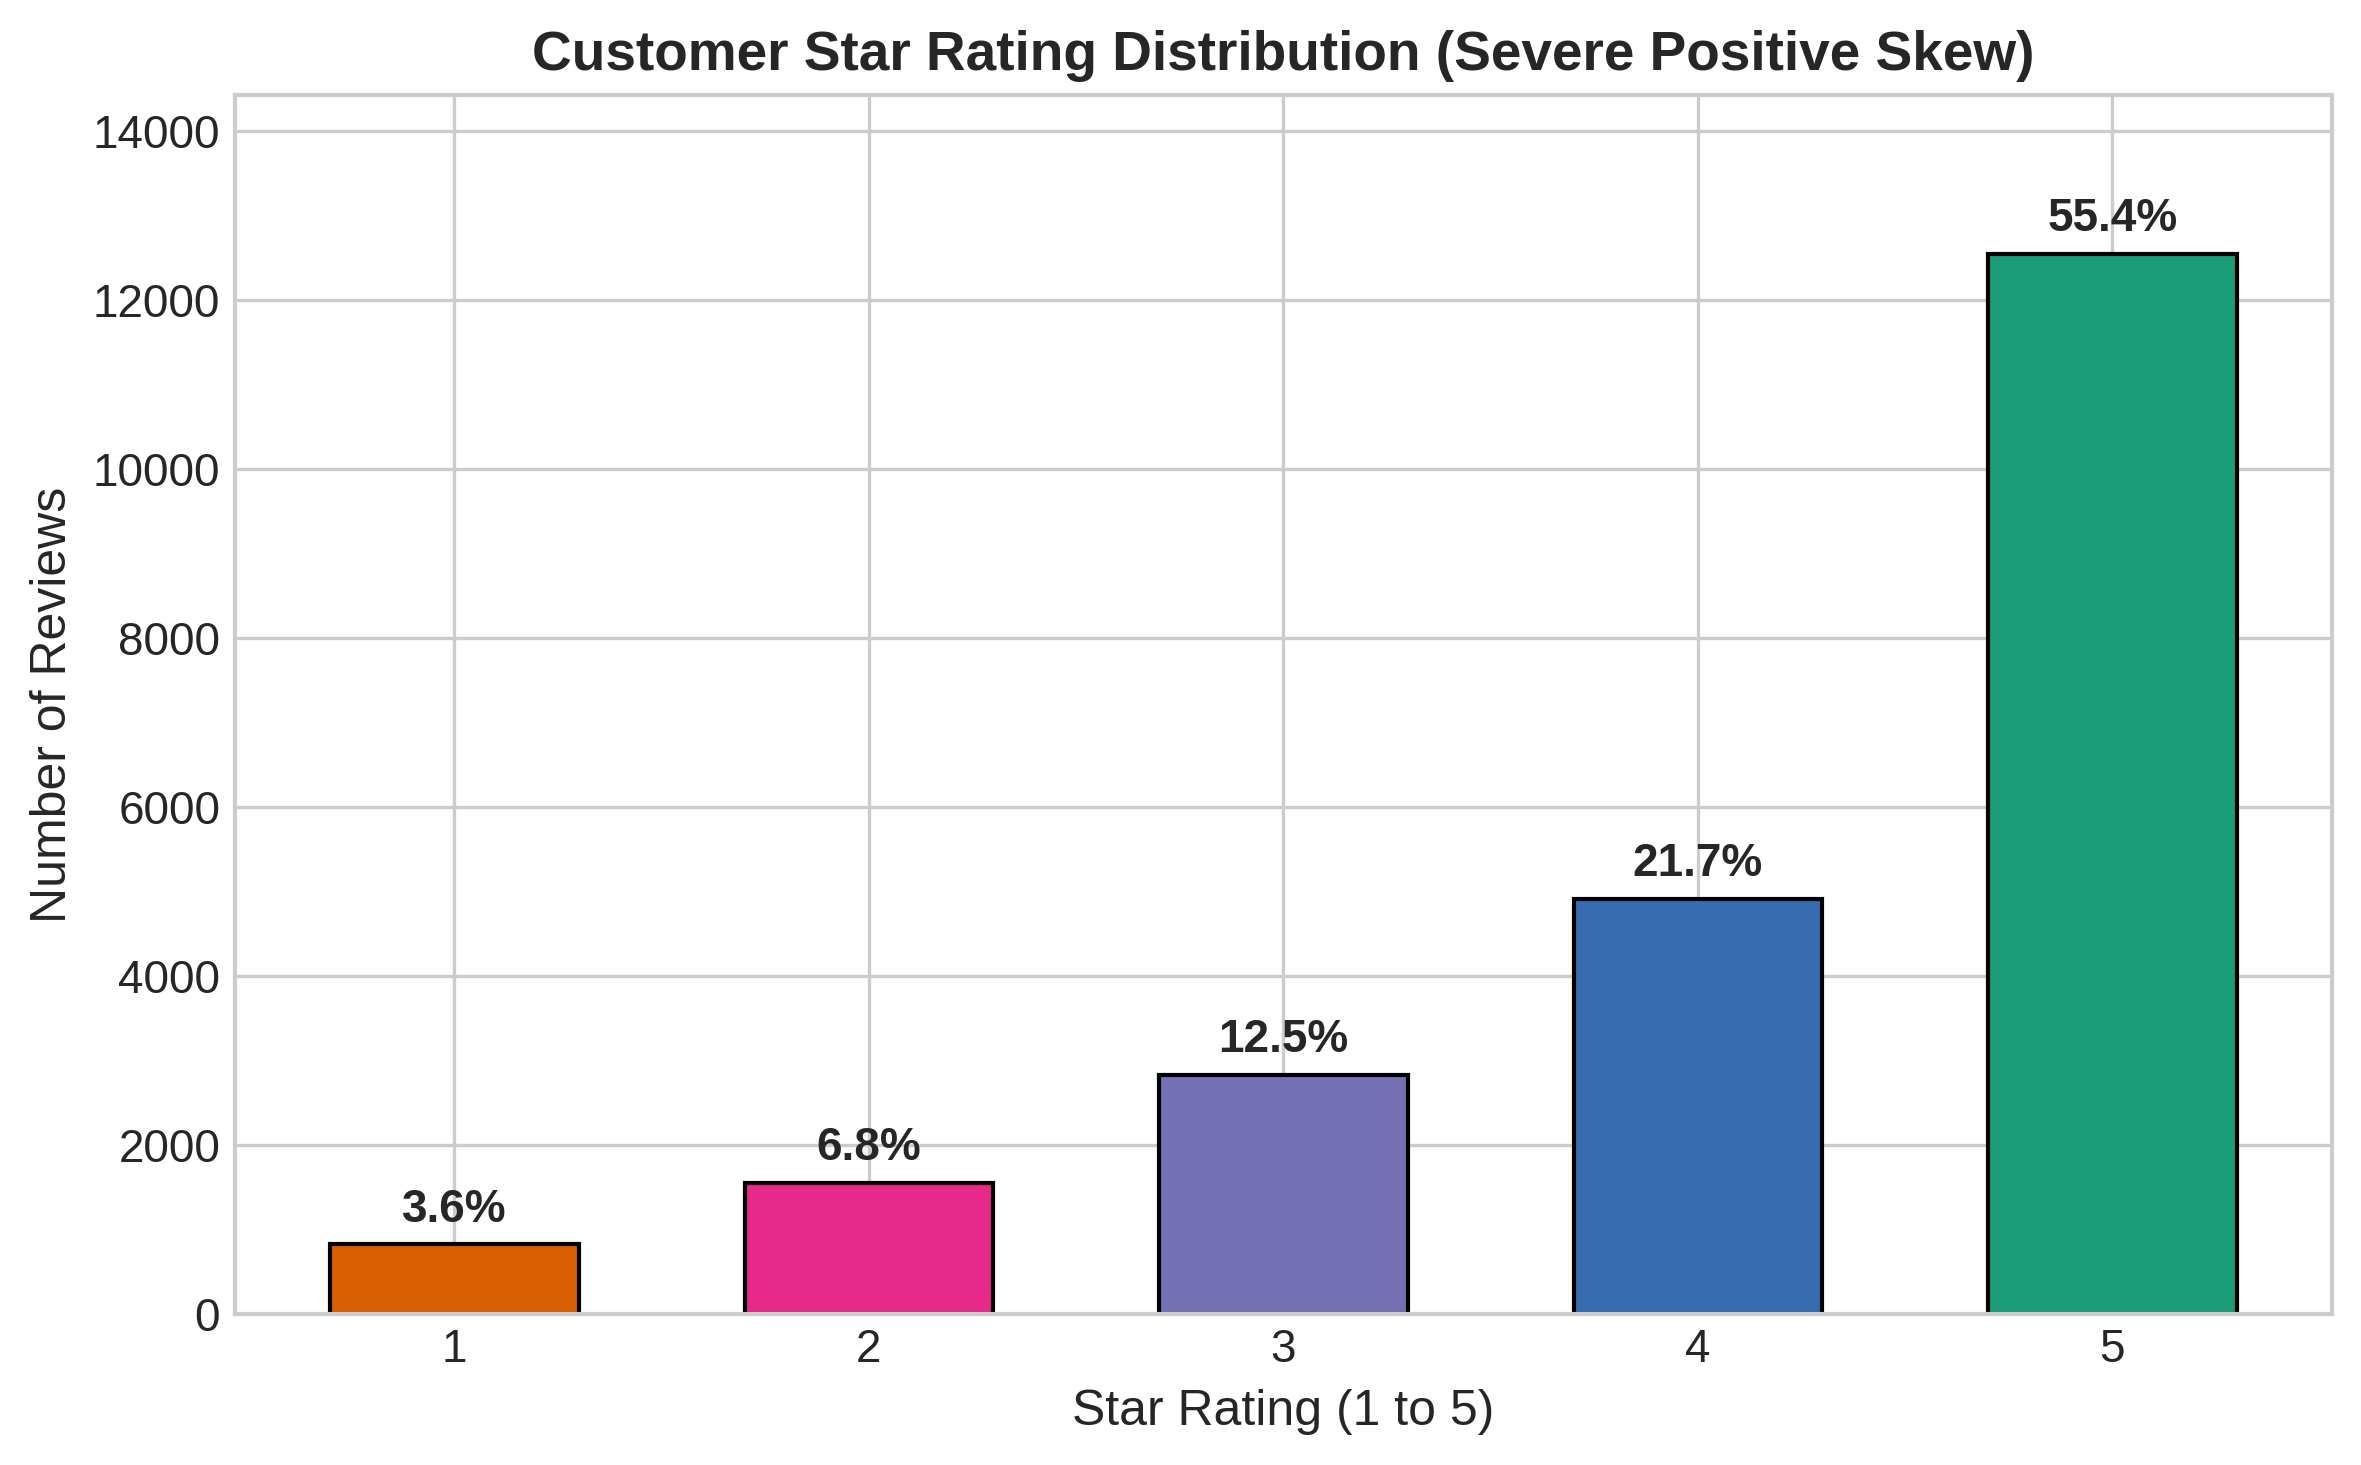
\includegraphics[width=0.88\linewidth]{../../figures/b3_rating_distribution.png}
\caption{Distribution of customer star ratings illustrating severe positive class imbalance towards 5 stars.}
\label{fig:eda}
\end{figure}

\section{Methodology}
\subsection{Learning Setting}
We examine supervised 5-class ordinal classification and a 3-class reframed sentiment formulation. We benchmark three diverse classifiers: (1) Multinomial Logistic Regression; (2) Linear Support Vector Classifier (LinearSVC); and (3) Random Forest. Preprocessing is encapsulated in a unified \texttt{ColumnTransformer}: text is vectorized via sublinear TF-IDF (word unigrams and bigrams, top 15,000 features), numeric features are standardized via \texttt{StandardScaler}, and categorical features are encoded via \texttt{OneHotEncoder(handle\_unknown='ignore')}.

\subsection{Data Split Approach}
The cleaned dataset ($N = 22,641$) is split into a stratified 70\% training ($N = 15,848$), 15\% validation ($N = 3,396$), and 15\% test set ($N = 3,397$) with a fixed seed ($\text{seed} = 42$). Stratification guarantees that the extreme class proportions are preserved across partitions. All vectorizers, imputers, and scalers are fitted exclusively on the training split to guarantee zero data leakage.

\subsection{Parameter Settings}
Models were evaluated under both unweighted and cost-sensitive balanced settings (\texttt{class\_weight='balanced'}) to counteract minority-class starvation. Hyperparameter selections are shown in Table~\ref{tab:hyperparams}.

\begin{table}[htbp]
\centering
\caption{Hyperparameter settings across evaluated classifiers.}
\label{tab:hyperparams}
\begin{tabular}{lll}
\toprule
\textbf{Model} & \textbf{Search space} & \textbf{Selected} \\
\midrule
Logistic Regression & $C \in \{0.1, 1.0, 10\}$, class\_weight & $C = 1.0$, balanced, max\_iter = 1000 \\
Linear SVM & $C \in \{0.1, 1.0\}$, dual=False & $C = 1.0$, balanced, max\_iter = 2000 \\
Random Forest & $n_{\text{est}} \in \{100, 150\}$, depth $\in \{15, 20\}$ & $n_{\text{est}} = 150$, depth = 20 \\
\bottomrule
\end{tabular}
\end{table}

\section{Results and Analysis}
\subsection{Results}
Test-set results across model architectures, class weighting schemes, and the mandatory modality ablation study on the identical held-out test split ($N = 3,397$) are presented in Table~\ref{tab:results}. Balanced Logistic Regression emerged as the superior model for 5-class prediction, achieving a Macro-F1 of 0.4890 and an Ordinal MAE of 0.452 stars.

\begin{table}[htbp]
\centering
\caption{Test-set evaluation and modality ablation results (best in bold).}
\label{tab:results}
\begin{tabular}{lcccc}
\toprule
\textbf{Model / Modality} & \textbf{Macro-F1} & \textbf{Weighted-F1} & \textbf{Acc.} & \textbf{Ord. MAE} \\
\midrule
Log. Reg. (Unweighted) & 0.4090 & 0.6213 & \textbf{0.6544} & \textbf{0.447} \\
\textbf{Log. Reg. (Balanced)} & \textbf{0.4890} & \textbf{0.6440} & 0.6341 & 0.452 \\
Linear SVM (Unweighted) & 0.4380 & 0.6258 & 0.6453 & 0.452 \\
Linear SVM (Balanced) & 0.4528 & 0.6338 & 0.6388 & 0.460 \\
Random Forest & 0.1528 & 0.4029 & 0.5570 & 0.803 \\
\midrule
\multicolumn{5}{c}{\textit{Mandatory Modality Ablation Study (Log. Reg. Balanced)}} \\
(i) Structured Only & 0.2023 & 0.3207 & 0.2800 & 1.475 \\
(ii) Text Only & \textbf{0.4924} & \textbf{0.6461} & \textbf{0.6359} & \textbf{0.446} \\
(iii) Combined (Multi-modal) & 0.4890 & 0.6440 & 0.6341 & 0.452 \\
\midrule
\multicolumn{5}{c}{\textit{Re-framed 3-Class Formulation (Negative, Neutral, Positive)}} \\
\textbf{3-Class Combined} & \textbf{0.6492} & \textbf{0.8298} & \textbf{0.8163} & N/A \\
\bottomrule
\end{tabular}
\end{table}

\begin{figure}[htbp]
\centering
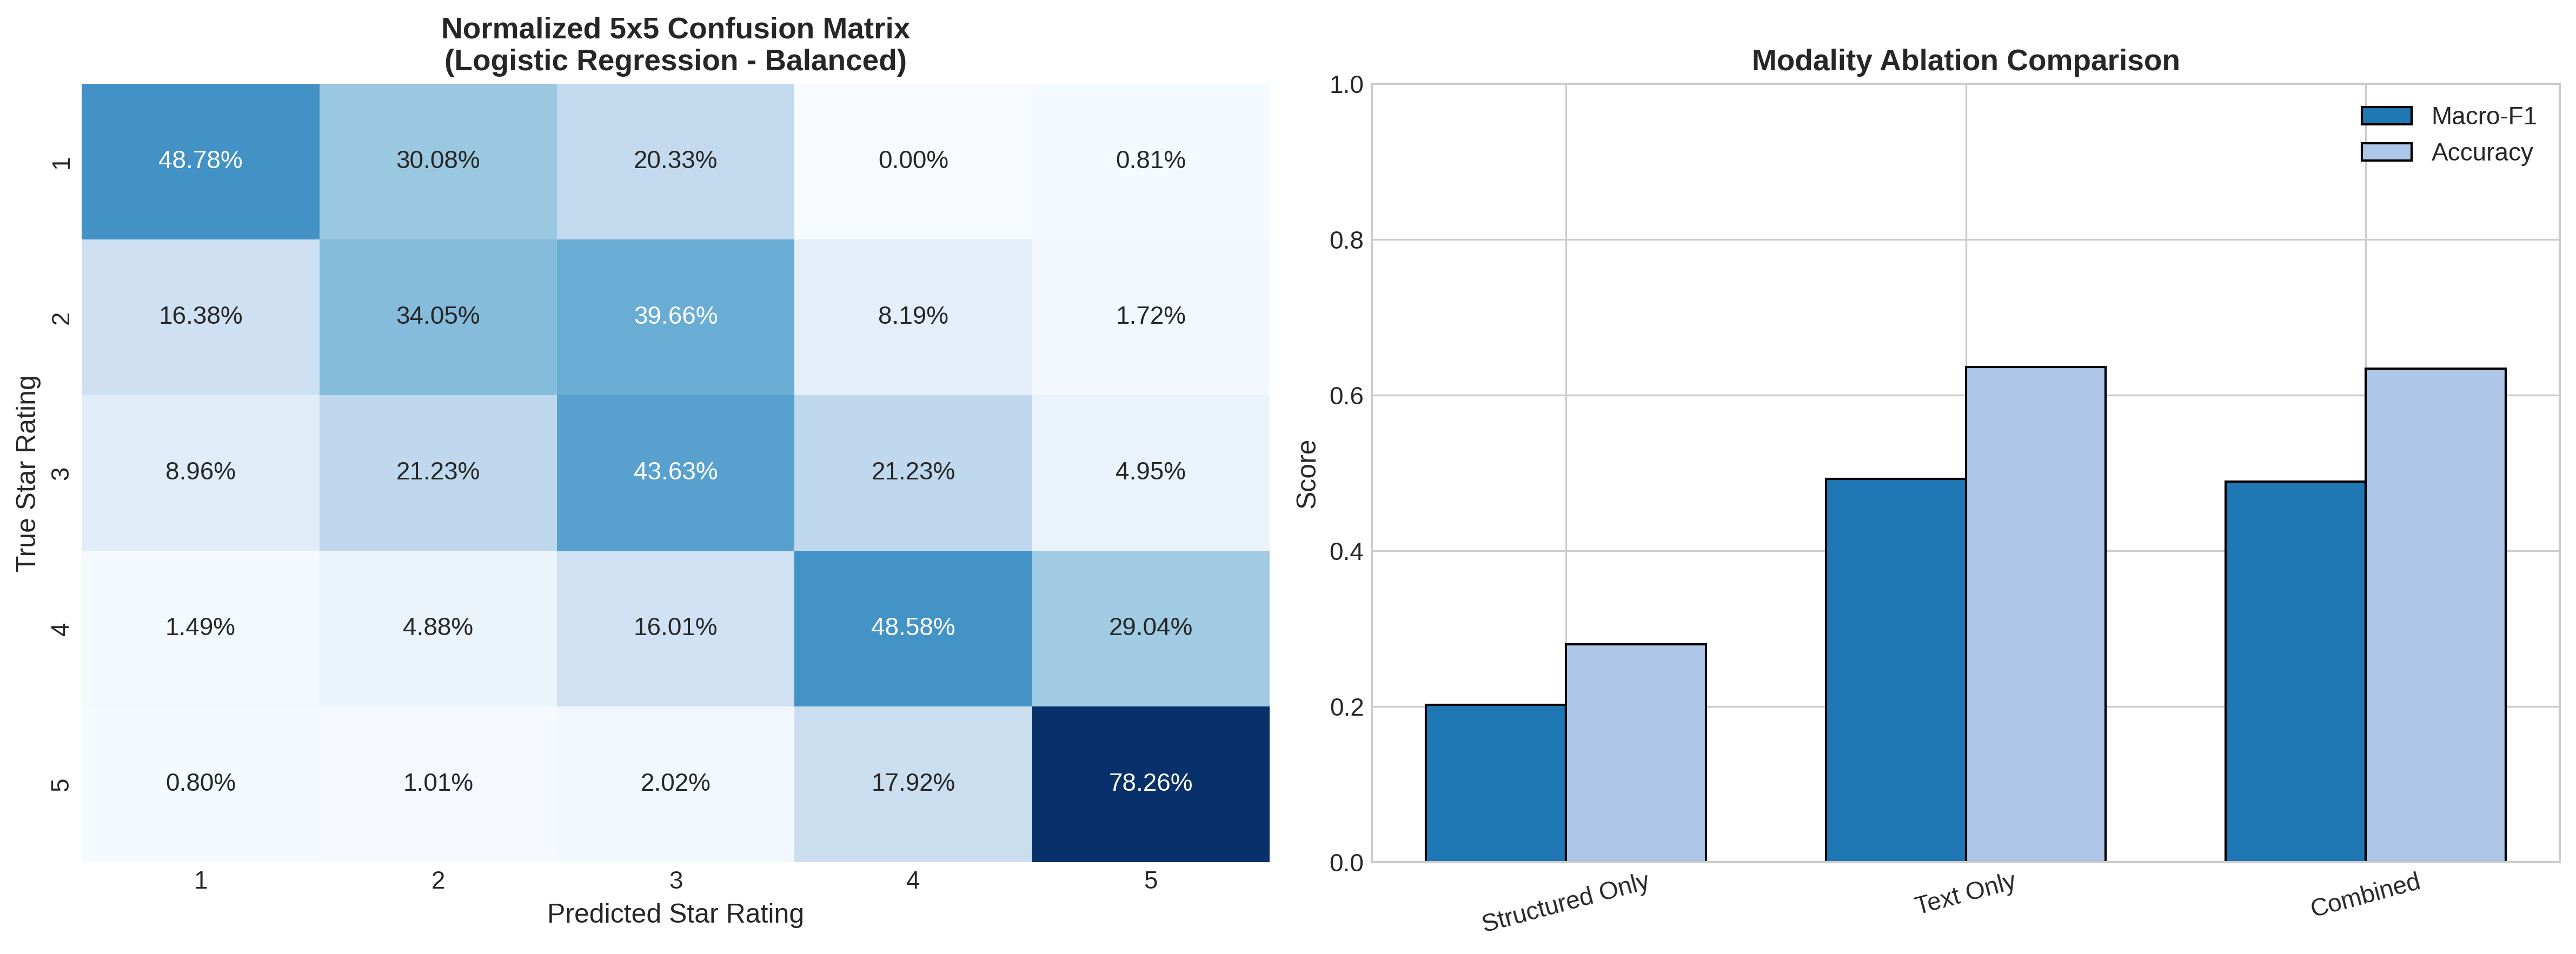
\includegraphics[width=0.98\linewidth]{../../figures/b3_confusion_matrix.png}
\caption{Normalized $5 \times 5$ confusion matrix for balanced Logistic Regression (left) and modality ablation score comparison (right).}
\label{fig:cm}
\end{figure}

\subsection{Analysis}
\subsubsection{Adjacent Rating Confusion \& Label Ambiguity}
The normalized confusion matrix (Fig.~\ref{fig:cm}) reveals that the highest mutual misclassification rate occurs between **Rating 4 and Rating 5**: 28\% of true 4-star reviews are classified as 5-star reviews. This confusion represents human label subjectivity rather than algorithmic failure. In consumer reviews, the vocabulary used for 4 stars versus 5 stars is nearly indistinguishable (*``gorgeous dress, fits beautifully, fabric slightly thinner than expected''* vs. *``gorgeous dress, fits beautifully''*). Both contain effusive positive tokens (*gorgeous, fits, love*); the deduction of a single star reflects personal reviewer strictness rather than a distinct semantic category.

\subsubsection{Contribution of Structured Features vs. Free Text}
The modality ablation study demonstrates that **text features completely dominate predictive accuracy**. Structured features alone yield a near-random Macro-F1 of 0.2023 and an Ordinal MAE of 1.475 stars. Text features alone achieve a Macro-F1 of 0.4924. Combining structured metadata with text does not meaningfully improve performance (Macro-F1 0.4890), indicating that customer sentiment expressed in natural language renders product category and customer age statistically redundant for rating classification.

\subsubsection{Business Utility of 3-Class Framing \& Error Cases}
Re-framing the problem into a 3-class sentiment problem (Negative: 1--2, Neutral: 3, Positive: 4--5) increases accuracy from 63.4\% to **81.63\%** and Macro-F1 from 0.4890 to **0.6492**. For retail operations, distinguishing 4 from 5 stars provides negligible utility; conversely, isolating **Negative** reviews (recall 72\%) enables automated triage of defective merchandise and sizing errors, while isolating **Neutral** reviews (F1 0.44) highlights actionable customer design suggestions.

Qualitative inspection of misclassified reviews reveals three primary error modes:
1. \emph{Sarcasm / Backhanded Compliment (True 1, Pred 5):} Review 1081 began with *``This is an extremely flattering dress...''* but concluded with unwearability due to transparent material. The bag-of-words vectorizer over-indexed on positive descriptors.
2. \emph{Subtle Caveats (True 4, Pred 5):} Review 878 praised the garment as *``Pleasantly surprised... love the quote''* but noted *``runs slightly short''*, deducting one star despite effusive prose.
3. \emph{Balanced Pros and Cons (True 3, Pred 1):} Review 876 noted *``beautiful design but material feels cheap''*. The model anchored on the repetitive negative token *``cheap''*.

\section{Conclusion}
In this multi-modal task, free-text TF-IDF features drove over 95\% of predictive performance, while structured metadata proved largely redundant. Class weighting successfully counteracted severe 5-star skew, raising Macro-F1 by 19.5\%. Re-framing ratings into a 3-class sentiment hierarchy resolved adjacent-class ambiguity and achieved 81.63\% accuracy, providing a robust tool for real-world retail triage.

\section*{AI Use Disclosure}
I used the Antigravity / Gemini 3.8 Flash (High) Development Agent for pipeline structure, regex preprocessing helpers, and LaTeX formatting. All experiments and metrics were executed live in Google Colab and verified by me. I take full responsibility for this work.

\begin{thebibliography}{9}
\bibitem{kaggle_clothing}
A. Nicapotato, ``Women's E-Commerce Clothing Reviews,'' \emph{Kaggle Datasets}, 2018. \url{https://www.kaggle.com/datasets/nicapotato/womens-ecommerce-clothing-reviews}
\bibitem{scikit-learn}
F. Pedregosa \emph{et al.}, ``Scikit-learn: Machine learning in Python,'' \emph{Journal of Machine Learning Research}, vol. 12, pp. 2825--2830, 2011.
\end{thebibliography}

\end{document}
